
\section{Introdução}




\noindent \begin{minipage}[c]{0.6\textwidth}
  \vspace {1cm}
\par Na disciplina de programação e desenvolvimento de banco de dados é apresentado aos discentes a linguagem \textbf{SQL} \textit{Structured Query Language}\ref{fig:logo}, para a manipulação desta linguagem é proposto o software \textbf{MySQL da Workbench}

\end{minipage}
\begin{minipage}[c]{0.4\textwidth}
  \captionof{figure}{Logo SQL}
  
\includegraphics[width=\textwidth]{figure/logo_sql.png}
  	\label{fig:logo}
    {\fontsize{10pt}{\baselineskip}\selectfont
    Fonte: \citeonline{logo:2023}
  }

\end{minipage}

\par Na figura \ref{fig:div_sql}, expõe a divisão da linguagem \textbf{SQL}, a mesma é dividida em cinco subconjuntos, sendo eles: \textbf{DQL \label{DQL}}, \textbf{DML}, \textbf{DDL \label{DDL}}, \textbf{DCL} e \textbf{DTL}, cada uma com suas respectivas funções. por exemplo a \textbf{DQL \ref{DQL}}, é a linguagem de consulta de dados, definida pelo comando \textit{SELECT}, ao qual possibilita a consulta do dados armazenados no banco de dados.

\begin{figure}[h!]
  \caption{Subdivisões da Linguagem SQL}
  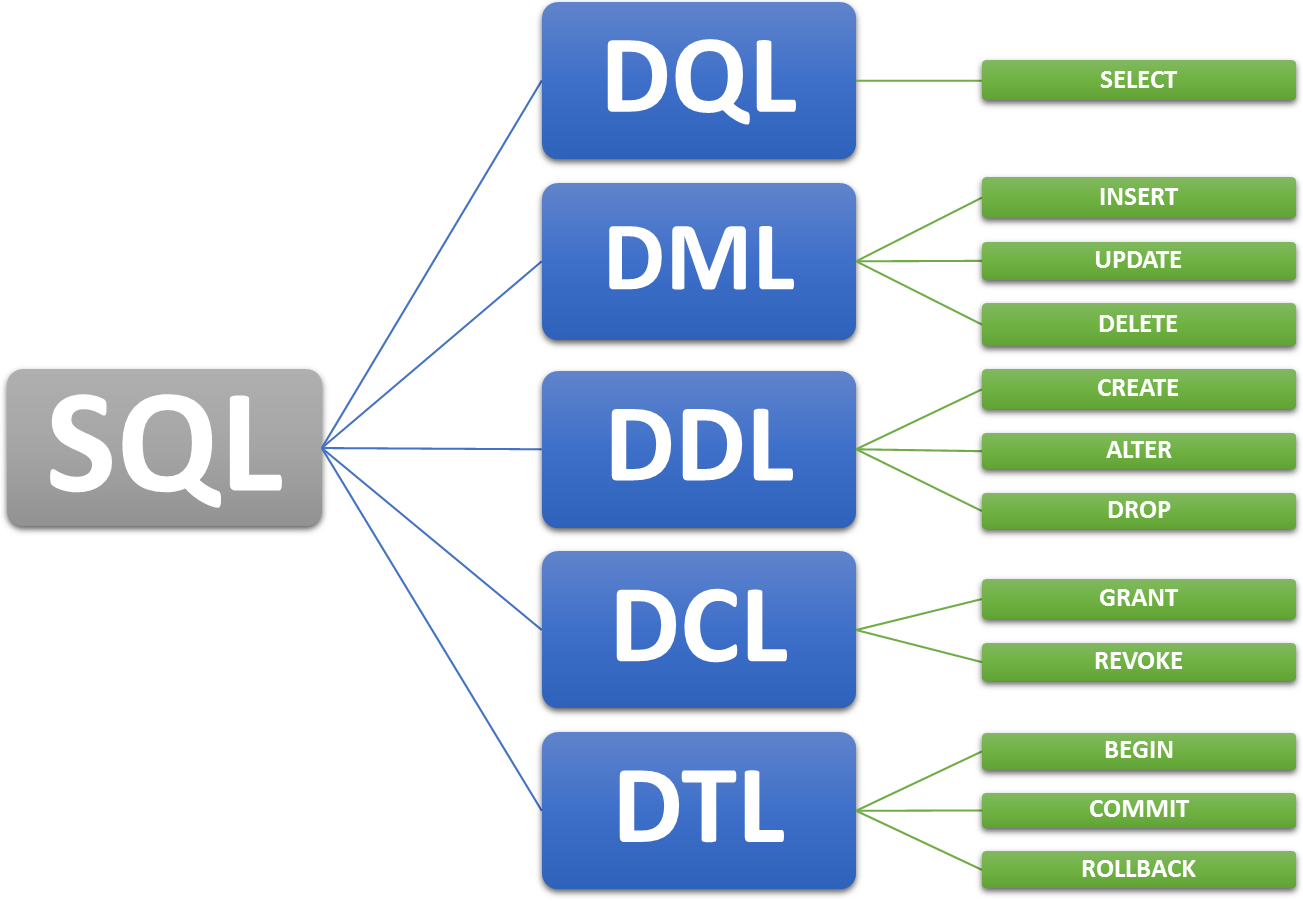
\includegraphics[width=\textwidth]{figure/div_SQL.png}
  \label{fig:div_sql}
  {\fontsize{10pt}{\baselineskip}\selectfont
  Fonte: \citeonline{guia:2023}  }
\end{figure}
\par Para esta aula prática é proposto o uso da \textbf{DDL}, Linguagem de definição de dados, a qual define os comandos \textit{CREATE}, \textit{ALTER} e \textit{DROP}, sendo elas na sequância, Criação de tabelas, visualzaões e índices; Alteração das estruturas e a remoção das estruturas criadas.

\section{Desenvolvimento}
\par Para implementação desta aula prática formam estabelecidos algumas regras informadas no roteiro \href{https://github.com/OgliariNatan/database_and_data_development/blob/main/aula%20pr%C3%A1tica.pdf}{da aula prática}. sendo a atividade proposta:
\begin{itemize}
  \item Criar uma estrutura de um banco de dados com a linguagem \textbf{SQL} por meio de uma entidade-relacionamento pré-definido;
  \item Inserir dados no banco de dados criado;
  \item Consultar os dados armazenados por meio da criação de uma visão (\textit{View});
  \item Elaborar um relatório no final da atividade;
\end{itemize}
\par Na atividade proposta o relatório dispõe de alguns procedimentos para a realização da atividade. Sugere a criação de uma base de dados de uma loja com o nome do banco de \textbf{Loja\_1}, com a utilizazão de definições de dados \textbf{DDL  \textsubscript{\ref{DDL}}} da linguagem SQL, e respeítando o modelo definido no \textbf{DER}, porposto pela atividade conforme figura \ref{fig:DER}.

\begin{figure}[h!]
  \caption{Diagrama entidade relacionamento}
  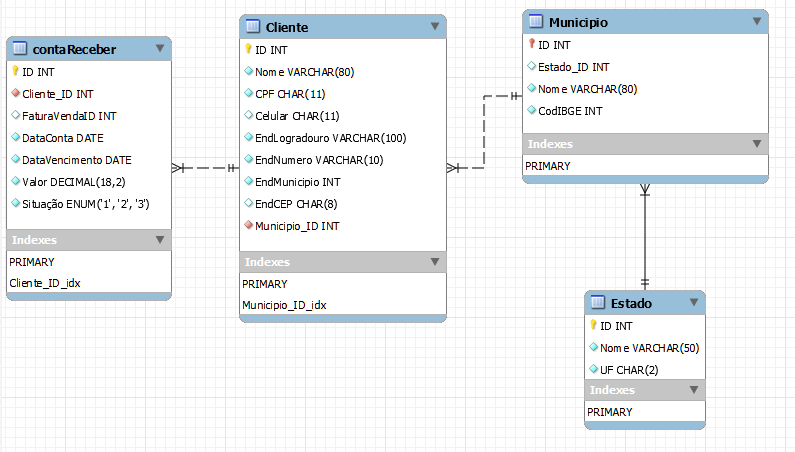
\includegraphics[width=\textwidth]{figure/diagram_EER.png}
  \label{fig:DER}
  {\fontsize{10pt}{\baselineskip}\selectfont
  Fonte: O autor (2023).}
\end{figure}

\par Uma observação importante o qual deprei no desenvolvimento desta atividade, foi que já possuia instalado o \textbf{MySQL da Workbench}, no entento, não estava configurado o SQL Server, portanto tive que configurar o mesmo.

\newpage

\section{Método}
\par Após a criação do projeto através do software \textbf{MySQL da Workbench}, foi proseguido com a criação do banco de bados conforme figura \ref{fig:DER}, com o estabelicimento de chaves primárias e as indicações de elementos não nulos e auto incrementais sendo quatro tabelas, em especifíco a tabela \textit{contaReceber}, possui um elemento chamdo de \textit{Situação ENUM('1', '2', '3')}, sendo: 1 - conta regitrada, 2 - conta cancelada e 3 - conta paga.


\par Deste modo é elaborado o \textit{scripty} Criação\_Loja\_1 conforme lista \ref{cod:cricao}, por segurança utilizo o especificador de banco o \textit{USE Loja\_1}.
\par Para a criação do Banco de dados \textbf{Loja\_1}, utilizei o metodo shell, e utlizei o scripty \autoref{cod:cricao}, específico o nome do banco e a codificação em \textit{utf8}. Para a criação das tabelas faz-se uso do operador \textit{IF NOT EXISTS}, para averiguação e caso já exista a tabela criada o mesmo não cria.

\lstinputlisting[caption={Criação\_Loja\_1.sql}, label={cod:cricao}]{criacao.sql}

\par A titulo de discussão no scripty \ref{cod:cricao}, a linha \textbf{52} está em comentário pois, acabei esquecendo de adiconar a linha \textit{Situação ENUM ('1', '2', '3') NOT NULL}, e para a correção exponho as linhas \textbf{59 a 62}\ref{cod:cricao}, para a correção deste lapso temporal. Neste ponto aproveito o aprendizado para a manipulação das tabelas com o comando \textbf{ALTER TABLE ... ADD}.

 \begin{figure}[h!]
 \caption{Captura de tela da criação do banco de dados.}
 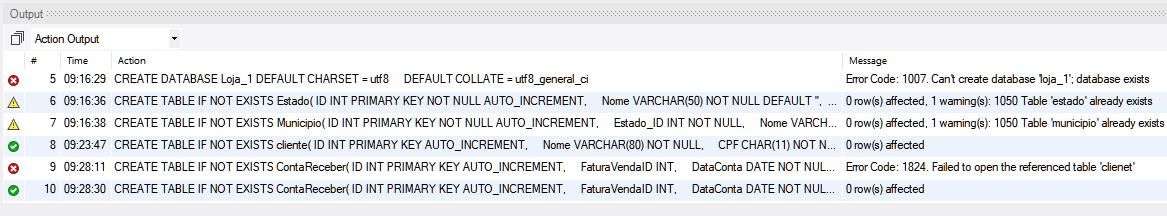
\includegraphics[width=\textwidth]{figure/fragmento.png}
 \label{fig:fragmento}
 {\fontsize{10pt}{\baselineskip}\selectfont
 Fonte: O autor (2023).}
 \end{figure}
\par Na Figura \ref{fig:banco}, expõe a captura de tela do banco de dados criado no MySql Workbench.
\newpage
 \begin{figure}[h!]
 \caption{Criação do banco de dados.}
 \begin{center}
    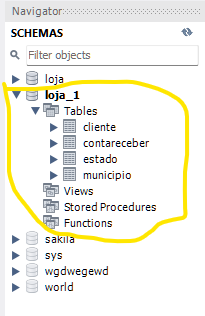
\includegraphics[scale=1]{figure/banco.png}
 \end{center}
 \label{fig:banco}
 {\fontsize{10pt}{\baselineskip}\selectfont
 Fonte: O autor (2023).}
 \end{figure}

\lstinputlisting[caption={inserir.sql}, label={cod:inserir}]{inserir.sql}

\par \textit{Scripty} para consulta de dados no banco de dados Loja\_1.

\lstinputlisting[caption={consulta.sql}, label={cod:consulta}]{consulta.sql}

\par O resultado do scripty \textit{consulta.sql} é demonstrado na figura \ref{fig:view}.

\begin{figure}[h!]
\caption{Visualização dos dados consutados}
\begin{center}
   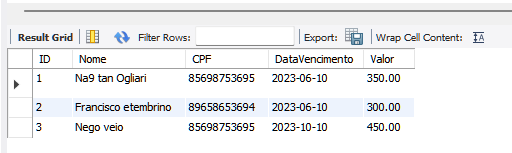
\includegraphics[scale=1]{figure/view.png}
\end{center}
\label{fig:view}
{\fontsize{10pt}{\baselineskip}\selectfont
Fonte: O autor (2023).}
\end{figure}

\par Desta forma é possível e necessario a criação de scripty para a manipulação dos dados armazenados.


\section{Conclusões}
\par A criação de um \textit{database}, parte de princípio melhoria no gerenciamento de dados de uma organização, e a criação de scripty de manipulação é necessário devido as suas progressivas e sucessivas necessidades de alterações, adicção, remoção e atualizações.
  %$X \xLongleftarrow[\text{NATAN}]{\text{OGLIARI}} Y $ %COM TEXTO
	% $\uparrow$ %Seta para Cima
	%$\overleftarrow{NATAN}$
